\PassOptionsToPackage{unicode=true}{hyperref} % options for packages loaded elsewhere
\PassOptionsToPackage{hyphens}{url}
\documentclass[11pt,dvipsnames,ignorenonframetext,aspectratio=169]{beamer}
\IfFileExists{pgfpages.sty}{\usepackage{pgfpages}}{}
\setbeamertemplate{caption}[numbered]
\setbeamertemplate{caption label separator}{: }
\setbeamercolor{caption name}{fg=normal text.fg}
\beamertemplatenavigationsymbolsempty
\usepackage{lmodern}
\usepackage{amssymb,amsmath}
\usepackage{ifxetex,ifluatex}
\usepackage{fixltx2e} % provides \textsubscript
\ifnum 0\ifxetex 1\fi\ifluatex 1\fi=0 % if pdftex
  \usepackage[T1]{fontenc}
  \usepackage[utf8]{inputenc}
\else % if luatex or xelatex
  \ifxetex
    \usepackage{mathspec}
  \else
    \usepackage{fontspec}
\fi
\defaultfontfeatures{Ligatures=TeX,Scale=MatchLowercase}







\fi

  \usetheme[]{monash}

  \usecolortheme{monashwhite}


% A default size of 24 is set in beamerthememonash.sty

% Title page
\setbeamertemplate{title page}
{\placefig{-0.01}{-0.01}{width=1.01\paperwidth,height=1.01\paperheight}{falcon.png}
\begin{textblock}{7.5}(1,2.8)\usebeamerfont{title}
{\color{white}\raggedright\par\inserttitle}
\end{textblock}
\begin{textblock}{7.5}(1,7)
{\color{white}\raggedright{\insertauthor}\mbox{}\\[0.2cm]
\insertdate}
\end{textblock}}


  \useinnertheme{rounded}

  \useoutertheme{smoothtree}

% use upquote if available, for straight quotes in verbatim environments
\IfFileExists{upquote.sty}{\usepackage{upquote}}{}
% use microtype if available
\IfFileExists{microtype.sty}{%
  \usepackage{microtype}
  \UseMicrotypeSet[protrusion]{basicmath} % disable protrusion for tt fonts
}{}


\newif\ifbibliography
  \usepackage[round]{natbib}
  \bibliographystyle{plainnat}


\hypersetup{
      pdftitle={Nanotechnology, definition, concepts and techniques},
            colorlinks=true,
    linkcolor=red,
    citecolor=Blue,
    urlcolor=lightgrayd,
    breaklinks=true}
%\urlstyle{same}  % Use monospace font for urls







% Prevent slide breaks in the middle of a paragraph:
\widowpenalties 1 10000
\raggedbottom

  \AtBeginPart{
    \let\insertpartnumber\relax
    \let\partname\relax
    \frame{\partpage}
  }
  \AtBeginSection{
    \ifbibliography
    \else
      \let\insertsectionnumber\relax
      \let\sectionname\relax
      \frame{\sectionpage}
    \fi
  }
  \AtBeginSubsection{
    \let\insertsubsectionnumber\relax
    \let\subsectionname\relax
    \frame{\subsectionpage}
  }



\setlength{\parindent}{0pt}
\setlength{\parskip}{6pt plus 2pt minus 1pt}
\setlength{\emergencystretch}{3em}  % prevent overfull lines
\providecommand{\tightlist}{%
  \setlength{\itemsep}{0pt}\setlength{\parskip}{0pt}}

  \setcounter{secnumdepth}{0}


%% Monash overrides
\AtBeginSection[]{
   \frame<beamer>{
   \frametitle{Outline}\vspace*{0.2cm}
   
   \tableofcontents[currentsection,hideallsubsections]
  }}

% Redefine shaded environment if it exists (to ensure text is black)
\ifcsname Shaded\endcsname
  \definecolor{shadecolor}{RGB}{225,225,225}
  \renewenvironment{Shaded}{\color{black}\begin{snugshade}\color{black}}{\end{snugshade}}
\fi
%%


  \usepackage{setspace}
  \usepackage{wasysym}
  % \usepackage{footnote} % don't use this this breaks all
  \usepackage{fontenc}
  \usepackage{fontawesome}
  \usepackage{booktabs,siunitx}
  \usepackage{longtable}
  \usepackage{array}
  \usepackage{multirow}
  \usepackage{wrapfig}
  \usepackage{float}
  \usepackage{colortbl}
  \usepackage{pdflscape}
  \usepackage{tabu}
  \usepackage{threeparttable}
  \usepackage{threeparttablex}
  \usepackage[normalem]{ulem}
  \usepackage{makecell}
  \usepackage{xcolor}
  \usepackage{tikz} % required for image opacity change
  \usepackage[absolute,overlay]{textpos} % for text formatting
  \usepackage{chemfig}
  \usepackage[skip=0.333\baselineskip]{caption}
  % \newcommand*{\AlignChar}[1]{\makebox[1ex][c]{\ensuremath{\scriptstyle#1}}}%

  % this font option is amenable for beamer
  \setbeamerfont{caption}{size=\tiny}
  \singlespacing
  \definecolor{lightgrayd}{gray}{0.95}
  \definecolor{skyblued}{rgb}{0.65, 0.6, 0.94}
  \definecolor{oranged}{RGB}{245, 145, 200}

  % \newlength{\cslhangindent}
  % \setlength{\cslhangindent}{1.5em}
  % \newenvironment{cslreferences}%
  %   {\setlength{\parindent}{0pt}%
  %   \everypar{\setlength{\hangindent}{\cslhangindent}}\ignorespaces}%
  %   {\par}


  \newcommand{\bcolumns}{\begin{columns}[T, onlytextwidth]}
  \newcommand{\ecolumns}{\end{columns}}

  \newcommand{\bdescription}{\begin{description}}
  \newcommand{\edescription}{\end{description}}

  \newcommand{\bitemize}{\begin{itemize}}
  \newcommand{\eitemize}{\end{itemize}}
  \AtBeginSubsection{}
  \usepackage{multicol}
  \usetikzlibrary{arrows.meta,positioning,shadings,shapes.geometric,calc}
  \usepackage{relsize}
  \tikzset{fontscale/.style = {font=\relsize{#1}}} % define a new style called 'fontscale', this uses 'relsize' package
  \usepackage{smartdiagram}

  \title[]{Nanotechnology, definition, concepts and techniques}


  \author[
        \vspace{-0.5cm}Deependra Dhakal\\
Assistant Professor\\
\textit{ddhakal.rookie@gmail.com}\\
\url{https://rookie.rbind.io}
    ]{\vspace{-0.5cm}Deependra Dhakal\\
Assistant Professor\\
\textit{ddhakal.rookie@gmail.com}\\
\url{https://rookie.rbind.io}}


\date[
      
  ]{
    }

\begin{document}

% Hide progress bar and footline on titlepage
  \begin{frame}[plain]
  \titlepage
  \end{frame}


   \frame<beamer>{
   \frametitle{Outline}\vspace*{0.2cm}
   
   \tableofcontents[hideallsubsections]
  }

\hypertarget{nanotechnology}{%
\section{Nanotechnology}\label{nanotechnology}}

\begin{frame}{}
\protect\hypertarget{section}{}
\bcolumns
\column{0.65\textwidth}
\small

\begin{itemize}
\tightlist
\item
  The term `nanotechnology' entered widespread use in late 1980s to
  describe anticipated technologies based on the use of molecule-based
  machine systems designed to build complex products with atomic
  precision.
\item
  Nanotechnology involves research and technology development at the
  1nm-100nm range (``nanodomain'').
\item
  Nanotechnology creates and uses structures that have
  ``\alert{novel properties}'' because of their small size and hence
  high surface area to volume ratio.
\item
  Builds on the ability to control or manipulate at the atomic scale.
\item
  Bacteria can be studied in a the scales of micro-meters. Viruses are
  in the order of 100nm.
\item
  The study of synthesis and characterization of nanomaterials is known
  as \alert{nanochemistry}.
\end{itemize}

\column{0.35\textwidth}

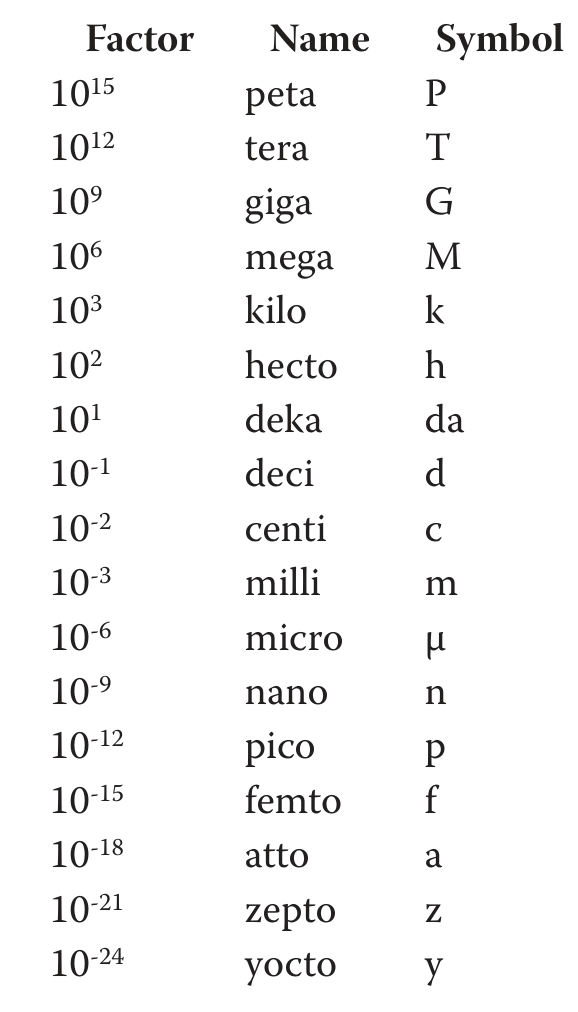
\includegraphics[width=0.7\linewidth]{../images/scale_distance}

\ecolumns
\end{frame}

\begin{frame}{Nanoscale effects}
\protect\hypertarget{nanoscale-effects}{}
\bcolumns
\column{0.3\textwidth}

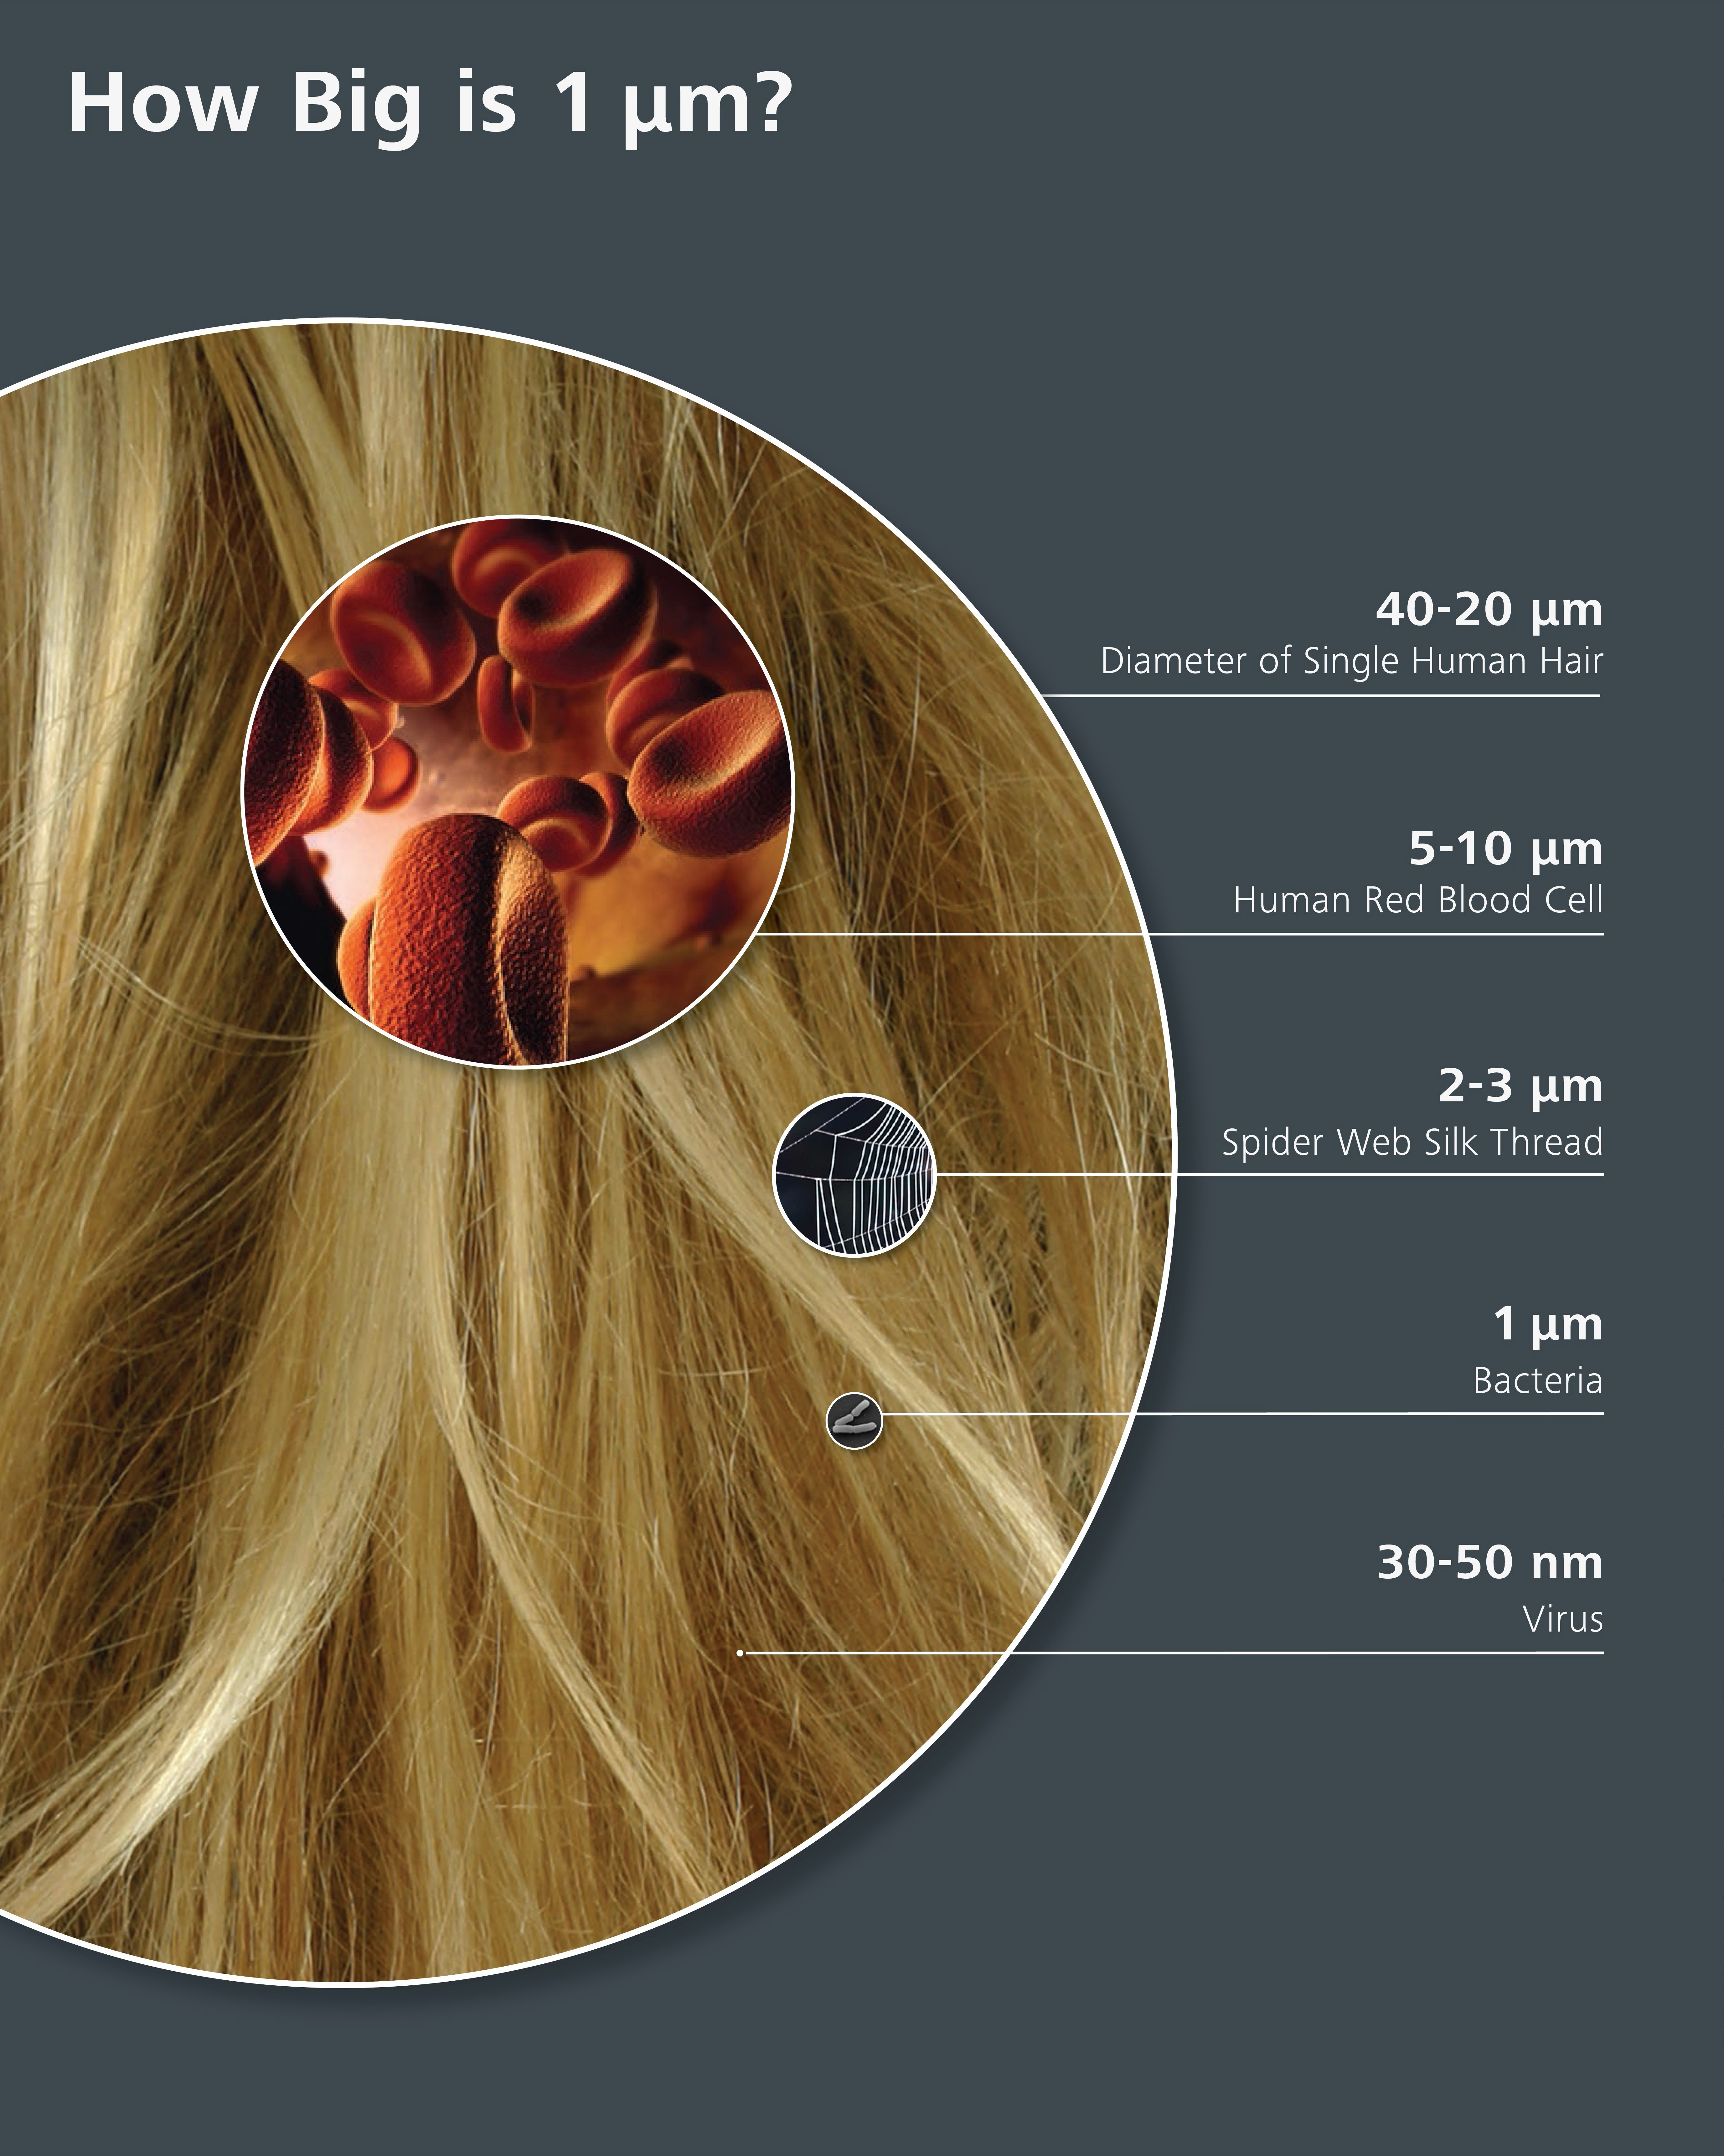
\includegraphics[width=0.98\linewidth]{../images/How_big_is_1_micrometer_wiki}

\column{0.4\textwidth}
\footnotesize

\begin{itemize}
\tightlist
\item
  On the one hand, the ratio of surface atoms to bulk atoms in
  nanoparticles is much more which may lead to situation where surface
  contributions predominate over bulk contributions to properties.
\item
  On the other hand, as particles become smaller and approach their
  \emph{de Broglie} wavelength (\(\lambda = \frac{h}{(mv)}\)), size
  effects become more evident because of quantum confinement. If the
  spacing between quantum levels (\(\Delta E\)) is higher than thermal
  excitation energy, i.e., \(\Delta E \geq k_B . T\), quantum effects
  predominate and size effects become very important.
\end{itemize}

\column{0.3\textwidth}

\begin{figure}
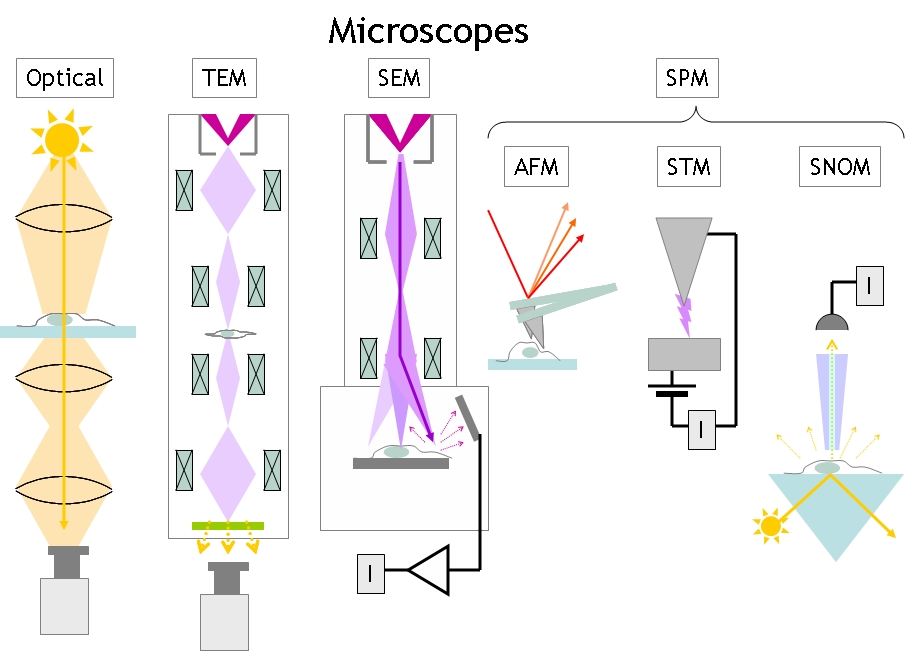
\includegraphics[width=0.98\linewidth]{../images/microscopes_overview} \caption{Overview of microscopy}\label{fig:microscopes-overview}
\end{figure}

\ecolumns
\end{frame}

\begin{frame}{}
\protect\hypertarget{section-1}{}
\begin{center}
\begin{tikzpicture}[scale=0.9]

\draw[thick,blue] (0,0) circle (4);

\begin{scope}

\clip (0,0) circle (4);
\foreach \i in {-360,-350,...,360}
{
\draw[blue] (\i:4) circle (2.5);
\draw[black] (\i+12:2) circle (2);
\draw[red] (\i+24:0.5) circle (1);

}

\end{scope}
\end{tikzpicture}
\end{center}
\end{frame}

\begin{frame}{Silicon nanowires}
\protect\hypertarget{silicon-nanowires}{}
\small

\begin{itemize}
\tightlist
\item
  Also referred to as SiNWs, these are a type of semiconductor nanowire
  most often formed from a silicon precursor by etching of a solid or
  through catalyzed growth from a vapor or liquid phase.
\item
  Applications in lithium ion batteries, thermoelectrics and sensors

  \begin{itemize}
  \footnotesize
  \item Experiment on nanowire solar cells has led to a remarkable improvement of the power conversion efficiency of SiNW solar cells from $\leq 1\%$ to $\geq 17\%$ in the last few years
  \item Exhibit charge trapping behavior which renders such systems of value in applications necessitating electron hole separation such as photovoltaics, and photocatalysts
  \item Possible use as metal insulator semiconductors and field effect transistors, with further applications as nanoelectronic storage devices, in flash memory, logic devices as well as chemical and biological sensors
  \end{itemize}
\item
  Features

  \begin{itemize}
  \footnotesize
  \item High electrical conductivity, owing to the bulk properties of doped Si, with low thermal conductivity due to the small cross section
  \item Unusual quasi one-dimensional electronic structure and are the subject of research
  \item Function as building blocks for nanoscale electronics assembled without the need for complex and costly fabrication facilities
  \end{itemize}
\end{itemize}
\end{frame}

\begin{frame}{Synthesis}
\protect\hypertarget{synthesis}{}
\footnotesize

\begin{enumerate}
\tightlist
\item
  Top down synthesis

  \begin{itemize}
  \scriptsize
  \item Laser beam ablation
  \item Ion beam etching
  \item Thermal evaporation oxide-assisted growth (OAG)
  \item Metal-assisted chemical etching (MaCE)
  \end{itemize}
\item
  Bottom-up synthesis

  \begin{itemize}
  \scriptsize
  \item Vapour liquid solid (VLS) growth - a type of catalysed CVD often using silane as Si precursor and gold nanoparticles as catalyst (or 'seed').
  \item Molecular beam epitaxy - a form of PVD applied in plasma environment
  \item Precipitation from a solution - A variation of the VLS method, aptly named supercritical fluid liquid solid (SFLS), that uses a supercritical fluid (e.g. organosilane at high temperature and pressure) as Si precursor instead of vapor. The catalyst would be a colloid in solution, such as colloidal gold nanoparticles, and the SiNWs are grown in this solution.
  \end{itemize}
\end{enumerate}

(Refer to the youtube Video -- How to grow silicon nanowires)
\end{frame}

\begin{frame}{Silver nanoparticles}
\protect\hypertarget{silver-nanoparticles}{}
\bcolumns
\column{0.6\textwidth}
\footnotesize

\begin{itemize}
\tightlist
\item
  Are nano-particles (1nm - 100nm) of Silver (\(\mathrm{Ag}\)) or silver
  oxide.

  \begin{itemize}
  \footnotesize
  \item over 300 nanosilver containing products have been identified, most of those marketed as dispersions and powder antimicrobials
  \end{itemize}
\item
  Numerous shapes can be constructed depending on the application --
  spherical, diamond, octagonal and thin sheets.
\item
  Large surface area permits the coordination of a vast number of
  ligands.
\item
  Nanomolecular silver solution reduced the incidence of root diseases.

  \begin{itemize}
  \tightlist
  \item
    use of a colloidal nanosilver solution may considerably improve the
    growth and health of various plants
  \end{itemize}
\end{itemize}

\column{0.4\textwidth}

\begin{figure}
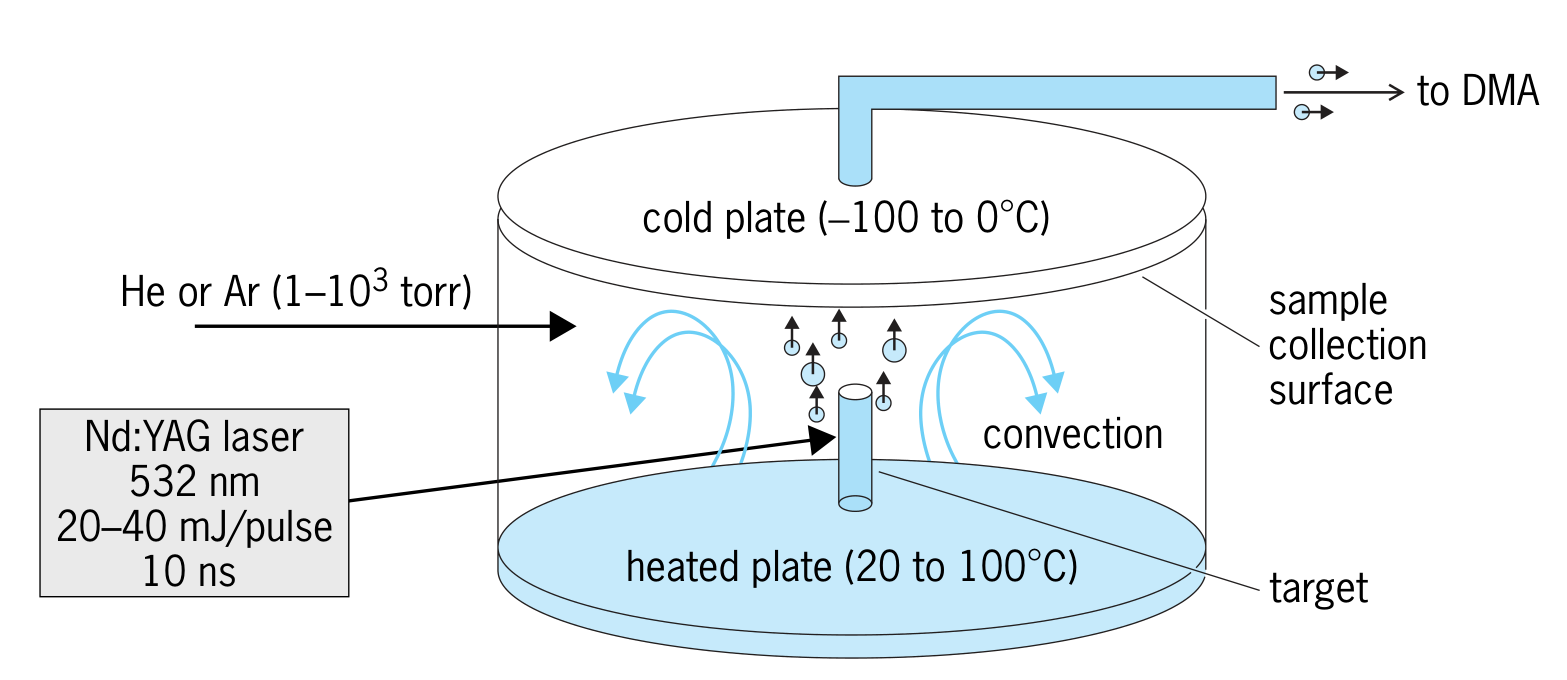
\includegraphics[width=0.75\linewidth]{../images/nanoparticles_synthesis_laser_vaporization} \caption{Experimental setup for the synthesis of nanoparticles by the laser vaporization controlled-condensation method coupled with a differential mobility analyzer (DMA) for the size selection of the nanoparticles. Common synthesis of metallic and intermetallic nanoparticles includes the decomposition of organometallic precursors, such as metal carbonyls (by thermal, photochemical, laser pyrolysis) to yield the respective element or alloys, and the reduction of inorganic or organometallic precursors by reducing agents. The size of the nanoparticle is determined by the particle residence time, temperature of the chamber, pressure and precursor composition. Vapor-phase synthesis of metallic nano-particles involves evaporation of the material followed by the condensation of clusters, ultimately giving off the nanoparticles from the vapor phase.}\label{fig:nanoparticle-synthesis-laser-vapor}
\end{figure}

\ecolumns
\end{frame}

\begin{frame}{Synthesis}
\protect\hypertarget{synthesis-1}{}
\footnotesize

\begin{itemize}
\tightlist
\item
  Precautions

  \begin{itemize}
  \scriptsize
  \item Wear lab coat, lab shoes, eye protection and follow the lab safety instructions
  \item Avoid light interaction with $\mathrm{Ag NO_3}$ solution 
  \end{itemize}
\item
  Requirements \setlength{\multicolsep}{4pt plus 1pt minus 1.5pt}

  \begin{multicols}{3}
  \begin{itemize}
  \setlength{\parskip}{0.1\baselineskip}
  \scriptsize
  \item Beaker
  \item Conical flask
  \item Magnetic stirrer
  \item Magnetic bead
  \item Burette
  \item Silver nitrate
  \item Deionized water
  \item Leaves of desired plants
  \end{itemize}
  \end{multicols}
\end{itemize}

\footnotesize

\begin{itemize}
\tightlist
\item
  Wash the fresh leaves of desired plant and cut in small pieces
\item
  Setup the magnetic stirrer
\item
  Take 25 g of leaves in 100 ml of DI water
\item
  Set the temperature to \SIrange{80}{90}{\celsius}
\item
  Filter the green extract in Burette to use as reducing and capping
  agent
\item
  Take 10mg \(\mathrm{Ag NO_3}\) in 50ml DI water (Caution: Cover the
  conical flask with aluminium foil to avoid photo-degradation of
  Silver.)
\item
  Set the temperature to \SIrange{60}{70}{\celsius}
\item
  Add leaf extract dropwise very slowly until the light yellow color
  forms.
\item
  The light yellow color in the solution is imparted by silver
  nano-particles.
\end{itemize}
\end{frame}

\begin{frame}{}
\protect\hypertarget{section-2}{}
\bcolumns
\column{0.5\textwidth}

\begin{itemize}
\tightlist
\item
  Carbon nano-tubes

  \begin{itemize}
  \tightlist
  \item
    Used for building molecular electronics
  \end{itemize}
\item
  Graphene

  \begin{itemize}
  \tightlist
  \item
    Derived from single sheet of carbon molecules
  \end{itemize}
\item
  Nanoparticles

  \begin{itemize}
  \tightlist
  \item
    Gold nono-paricles for medical imaging
  \end{itemize}
\end{itemize}

\column{0.5\textwidth}

\begin{figure}
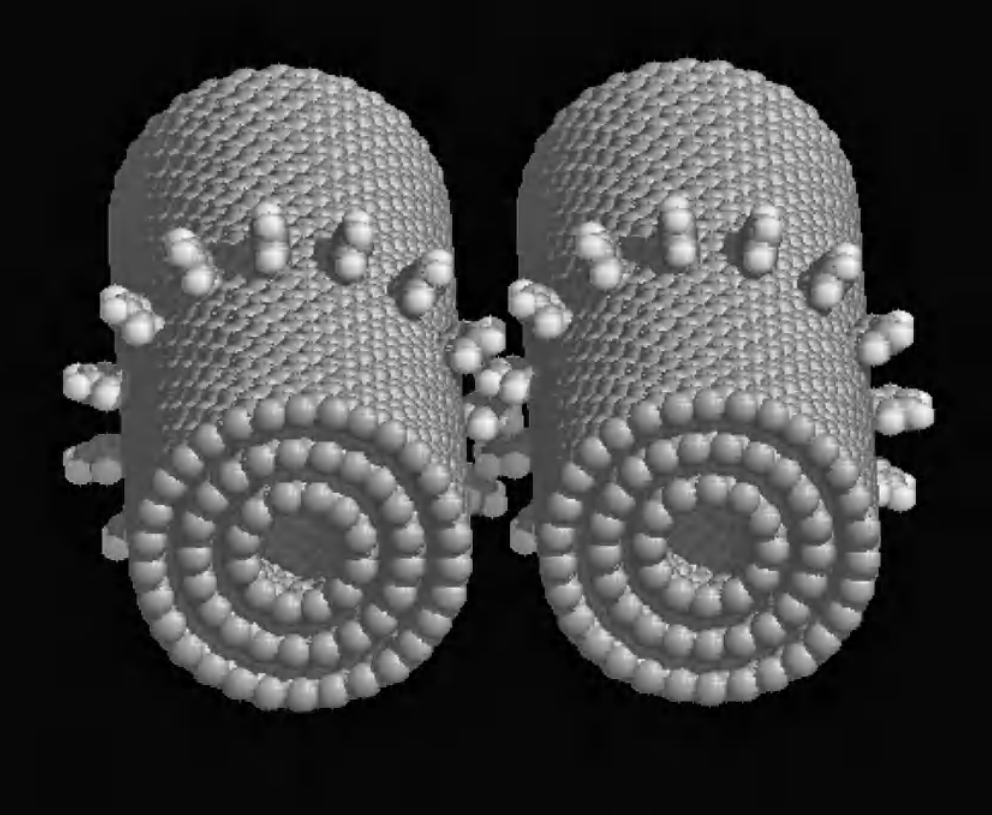
\includegraphics[width=0.7\linewidth]{../images/carbon_nanotubes} \caption{Simulation of a carbon nanotube-based gear.}\label{fig:carbon-nanotubes}
\end{figure}

\ecolumns
\end{frame}

\begin{frame}{Silicon nano-particles (nano-crystallites or quantum
dots)}
\protect\hypertarget{silicon-nano-particles-nano-crystallites-or-quantum-dots}{}
\begin{itemize}
\tightlist
\item
  Unlike bulk silicon (a dull material, inefficient at emitting light),
  ultrasmall silicon nano-particles are spectacularly efficient at
  emitting light in RGB colors.
\item
  Sleuth of interests in silicon nanotechnology came nearly a decade
  after the exciting discover by Canham in 1990 of visible red
  photoluminescence (PL) at room temperature with a quantum efficiency
  of few percent, from electrochemically etched silicon (porous silicon
  (PS) layer).
\item
  The research led by Nayfeh at Illinois in 2000 has shown that reducing
  the size of an elemental Si crystal to a few tens of atom
  (\textasciitilde1nm), without altering its chemical composition,
  effectively creates a new material, a nanoparticle with novel
  properties - both electronic and non-electronic, including ultrabright
  ultrastable luminescence.
\end{itemize}
\end{frame}

\hypertarget{applications-of-nano-technology}{%
\section{Applications of
nano-technology}\label{applications-of-nano-technology}}

\begin{frame}{}
\protect\hypertarget{section-3}{}
\begin{center} % center makes standalone package go berserk! don't use with it.
% scaling of 'every node/.style' will scale the bounding draws as well.
% to scale fonts only create a font style

%\begin{tikzpicture}[every node/.style={scale=0.8}]
\begin{tikzpicture}[scale=0.8, every node/.style={scale=0.4}]

%\draw[step=0.5cm,very thin,black!20] (-6,-6) grid (6,6);

\node[shape=circle, draw=black, text width=2cm, fill=red!20, align=center] (cropsoil) at (0,0) {\small Enhance crop production and soil health};

% anchor is obtained from positioning library
\tikzstyle{technologybox}=[shape=rectangle, draw=blue, anchor=west, fontscale=0.6, text width=2cm, align=center]

\node[technologybox] (A) at (2,2) {Nanofertilizers};
\node[technologybox] (B) at (2,0.5) {Nanopesticides};
\node[technologybox] (C) at (2,-0.5) {Nanobiosensors};
\node[technologybox] (D) at (2, -2) {Nano-enabled remediation of contaminated soils};

\draw[<-] (cropsoil) -- (A);
\draw[<-] (cropsoil) -- (B);
\draw[<-] (cropsoil) -- (C);
\draw[<-] (cropsoil) -- (D);

% \draw[top color=blue!30] (-5,3) rectangle (-3,-3);

\tikzstyle{appliedoutbox}=[shape=rectangle, draw=black, anchor=mid, fontscale=0.7, text width=2.5cm, align=center, rounded]

\node[technologybox] (A1) at (-4,2) {Food technology};
\node[technologybox] (B1) at (-4,0.5) {Biotechnology and genetics};
\node[technologybox] (C1) at (-4,-0.5) {Agronomy and crop physiology};
\node[technologybox] (D1) at (-4,-2) {Soil management and crop nutrition};

\tikzstyle{appliedoutboxbranch}=[shape=rectangle, text width=3cm, fontscale=0.8, align=center, draw=red, scale=0.6]

\node[appliedoutboxbranch, anchor=north] (A11) at (-1,4) {Encapsulement and delivery of materials, flavor development, introducing nano-antimicrobials agents into food, shelf life enhancement, contamination sensing, improved food preservative, monitoring, tracing};
\node[appliedoutboxbranch] (B11) at (-5,1) {Gene delivery, genetic transformation, RNAi};
\node[appliedoutboxbranch] (C11) at (-5,-1) {Enhanced germination, improved seedling vigor better tolerance to stress};
\node[appliedoutboxbranch, anchor=south] (D11) at (-1,-4) {Mineral chelation, improvement of soil physical property, reduced nutrient loss and synergistic effects with soil nutrients};

\draw[<-] (A1) -- (cropsoil);
\draw[<-] (B1) -- (cropsoil);
\draw[<-] (C1) -- (cropsoil);
\draw[<-] (D1) -- (cropsoil);

\draw[<-] (A11) -- (A1);
\draw[<-] (B11) -- (B1);
\draw[<-] (C11) -- (C1);
\draw[<-] (D11) -- (D1);

\end{tikzpicture}
\end{center}
\end{frame}

\begin{frame}{Benefits to crops}
\protect\hypertarget{benefits-to-crops}{}
\begin{enumerate}
\tightlist
\item
  Better root growth
\item
  Better shoot growth
\item
  Larger leaves and vegetative parts
\item
  Higher photosynthetic rate
\end{enumerate}

\begin{itemize}
\tightlist
\item
  \(\uparrow\) Fruit and seed yield
\item
  \(\uparrow\) Biomass \(\therefore\) better carbon assimilation
\end{itemize}

\begin{enumerate}
\setcounter{enumi}{4}
\tightlist
\item
  High concentration of minerals
\end{enumerate}
\end{frame}

\begin{frame}{In-situ hybridization}
\protect\hypertarget{in-situ-hybridization}{}
\bcolumns
\column{0.55\textwidth}
\footnotesize

\begin{itemize}
\tightlist
\item
  Fluorescence microscopy is often used to detect specific proteins or
  other molecules in cells and tissues.
\item
  Fluorescent dyes couple with antibody molecules, the distribution of
  the latter can be visualized when dye, for example, \emph{fluorescein}
  is excited with the blue light, which emits an intense green
  fluorescence.
\item
  Organic fluorochromes fade rapidly when continuously illuminated.
\item
  Nanoparticles can be excited to fluoresce \emph{more stably} by a
  broad spectrum of blue light, with their light emission depending on
  the exact size of the nanocrystal.

  \begin{itemize}
  \scriptsize
  \item  If introduced into a living cell, in an embryo for example, the progeny of that cell can be followed many days later by their fluorescence, allowing cell lineages to be tracked.
  \end{itemize}
\end{itemize}

\column{0.45\textwidth}

\begin{figure}
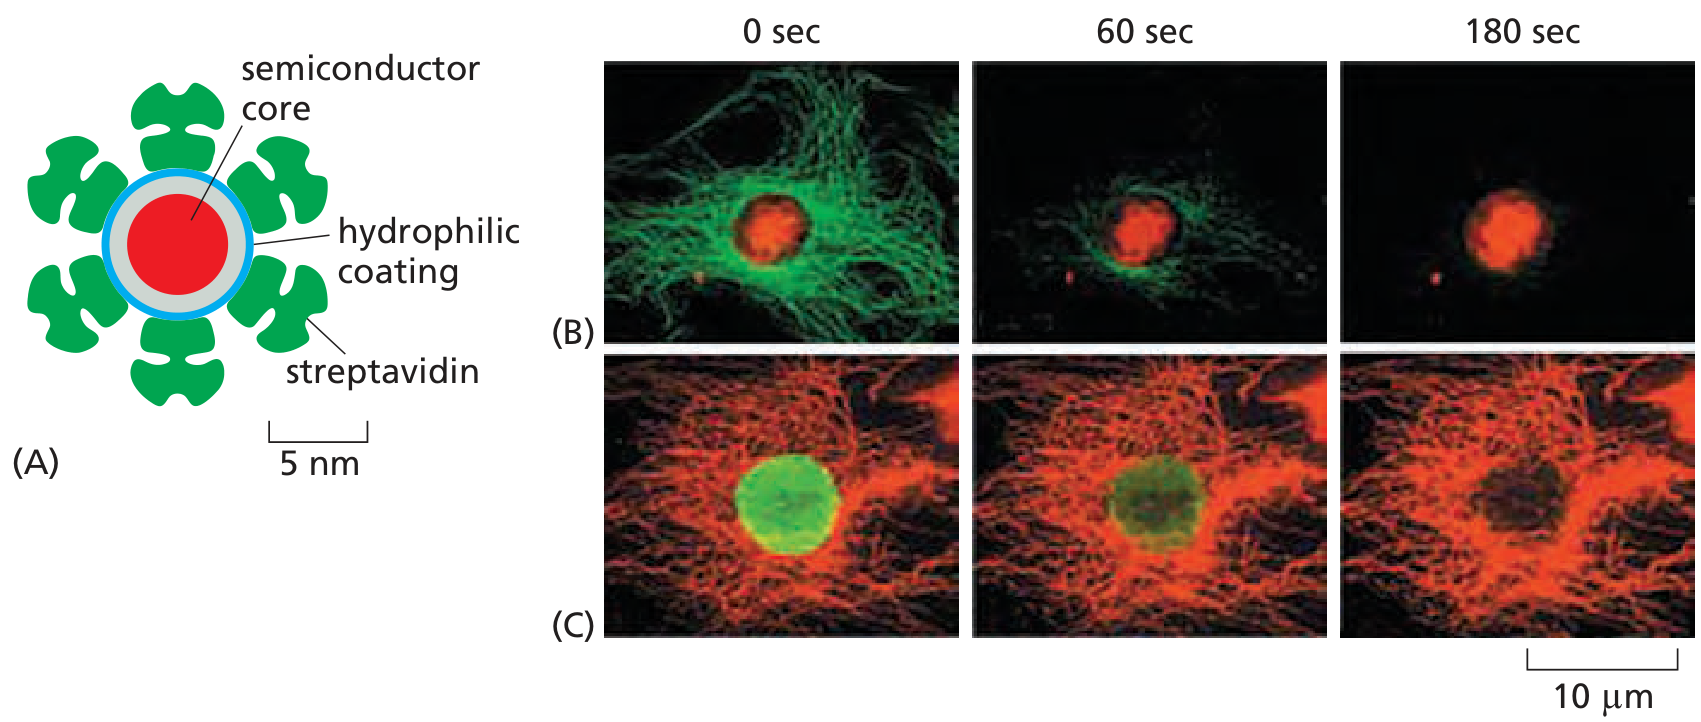
\includegraphics[width=0.98\linewidth]{../images/nanoparticles_fluorescent_dyes} \caption{Fluorescent nanoparticles. (A) Quantum dots are tiny particles of cadmium selenide, a semiconductor, with a coating to make them water-soluble. They can be coupled to protein molecules such as antibodies or streptavidin and, when introduced into a cell, will bind to a target protein of interest. Different-sized quantum dots emit light of different colors -- the larger dot, the longer the wavelength -- but they are all excited by the same blue light. They can continue to fluoresce for weeks, unlike most organic fluorescent dyes. (B) In this cell, microtubules are labelled (green) with an organic fluorescent dye (Alexa 488), while a nuclear protein is stained (red) with quantum dots bound to streptavidin. On continuous exposure to strong blue light, the fluorescent dyes fade quickly while the quantum dots continue to shine. (C) In this cell, the labelling pattern is reversed. Again, the quantum dots far outlast the fluorescent dye.}\label{fig:nanoparticles-fluorescent-dyes}
\end{figure}

\ecolumns
\end{frame}

\begin{frame}{Gene delivery}
\protect\hypertarget{gene-delivery}{}
\footnotesize

\begin{itemize}
\tightlist
\item
  Gene delivery systems are essential components of genetic medicine. It
  involves the transport of genes, which requires a transport vehicle
  referred to as a \alert{vector}. Possible vectors include viral
  ``shells'' or lipid spheres (Liposomes), which have properties that
  allow them to be incorporated into host cells.
\item
  Current genetic therapies are targeted towards
\item
  Mesoporous silica nano-particles (MSNs) have been extensively
  investigated as a drug delivery system, due to its high specific area,
  high pore volume, tunable pore structure and physicochemical
  stability.

  \begin{itemize}
  \footnotesize
  \item delivery of both hydrophilic or hydrophobic active agents
  \item delivery of DNA and chemicals into isolated plant cells by coating MSNs
  \item MPS/DNA complexes showed enhanced transfection efficiency through receptor-mediated endocytosis via mannose receptors of the cell wall
  \end{itemize}
\item
  To date, gene editing has become mediated mostly by viral vectors;
  however, inorganic nanoparticles lately received great importance as
  carriers for gene delivery or editing systems such as CRISPR. They
  signify a promising nano-biology tool to transfer some biomolecule
  such as DNA, RNA, and protein to the targeted plant cells, because of
  their capability to transport large sizes once used as a vehicle.
\end{itemize}
\end{frame}

\begin{frame}{Nano-enabled remediation}
\protect\hypertarget{nano-enabled-remediation}{}
\bcolumns
\column{0.55\textwidth}
\footnotesize

\begin{itemize}
\tightlist
\item
  Materials such as metal and metal oxide/sulphide allomorphs, polymers,
  carbon allotropes, etc. may be transformed, doped or prepared in
  different morphologies (sizes and shapes), with a variety of surface
  characteristics.
\item
  Active surface and the number of reactive sites on the surface or the
  porosity, all related to surface phenomena, have wide range of
  applications that benefit from nanometric size.
\item
  Persistent and mobile organic compounds (PMOCs) that pose serious
  health and environment risks are shown to be effectively managed in
  adsorption and redox processes through the use of nanomaterials.
\end{itemize}

\begin{center}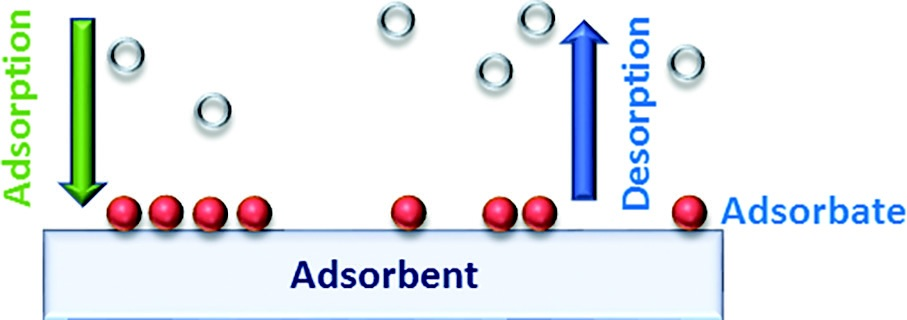
\includegraphics[width=0.55\linewidth]{../images/environmental_remediation_nanoparticles} \end{center}

\column{0.45\textwidth}

\begin{figure}
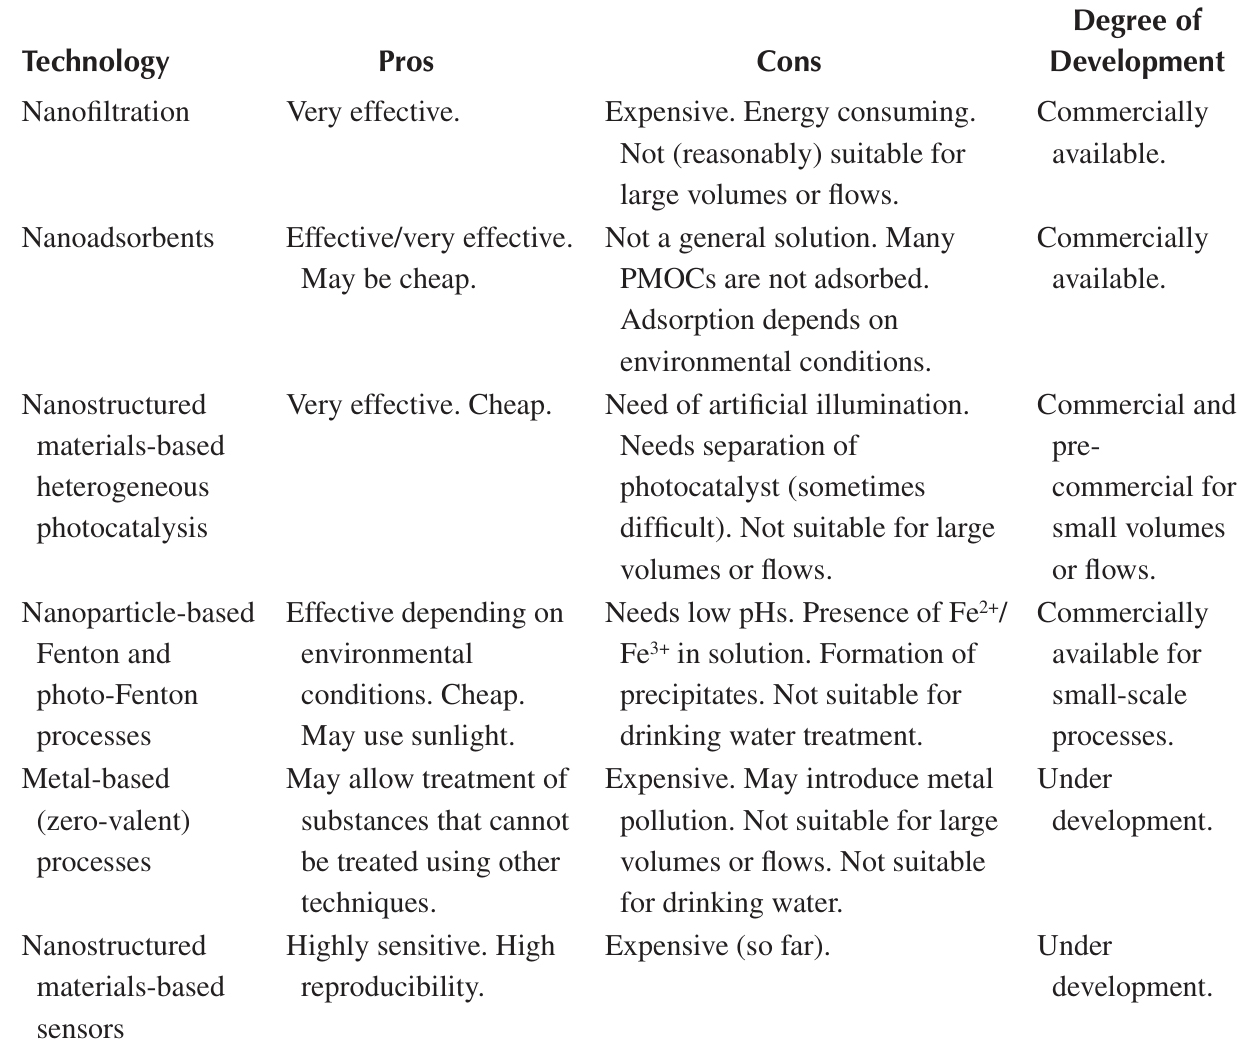
\includegraphics[width=0.88\linewidth]{../images/nano_technology_solution_water} \caption{Nano-material based technologies used nowadays in water treatment.}\label{fig:nano-technology-water}
\end{figure}

\ecolumns
\end{frame}

\begin{frame}{Nanosensors}
\protect\hypertarget{nanosensors}{}
\begin{itemize}
\tightlist
\item
  Biosensors have been around since glucose monitors were commercialized
  in the 1970s, but translation into commercial world of major ideas
  from nanotechnology has lagged.
\item
  Nanomaterials has increasing value for use as electrochemical
  biosensors due to high sensitivity and fast response times.

  \begin{itemize}
  \tightlist
  \item
    effective immobilization of biomolecules without altering
    bioactivity is the key in construction of stable and well-structured
    electrode material for biosensor platform
  \end{itemize}
\item
  Biosensor systems are ideal tool for real-time monitoring of
  organophosphate pesticides and nerve agents.
\item
  Bioananalytical nanosensors can be utilized to detect and quantify
  presence of contaminants (virus, bacteria, toxins) in trace amounts in
  food and agriculture systems.
\end{itemize}
\end{frame}

\begin{frame}{Agronomy and crop physiology}
\protect\hypertarget{agronomy-and-crop-physiology}{}
\begin{itemize}
\tightlist
\item
  Silver (\(\mathrm{Ag}\)) nanoparticles \(\longrightarrow\) seed
  priming of Jasmine \(\longrightarrow\) \(\uparrow\) Germination \%.
\item
  \(\mathrm{FeS_2}\) \(\longrightarrow\) \(\uparrow\) Stress tolerance
\item
  Cesium oxide (\(\mathrm{CeO_2}\)) \(\longrightarrow\) \(\downarrow\)
  Germination \% in Radish and Spinach

  \begin{itemize}
  \tightlist
  \item
    Antioxidants (Catalase, superoxide dismutate,
    glutathione-peroxidase) reduce the activity of amylase. Like organic
    counterparts, \(\mathrm{CeO_2}\) acts effectively as autocatalytic
    anti-oxidant thus inhibiting activity of amylase required for
    promotion of germination.
  \end{itemize}
\item
  Carbon nanotube applied on onion promoted root growth development.
\item
  Starch accumulation of fruit and root biomass of cucumber was
  positively affected by \(\mathrm{ZnO}\).
\item
  \(\mathrm{Zn}\) fortified core with \(\mathrm{MnCO3}\) nano-shell when
  applied to soil in rice fields increased the production.
\end{itemize}
\end{frame}

\begin{frame}{Nano-fertilizers}
\protect\hypertarget{nano-fertilizers}{}
\begin{center}
\tikzstyle{block}=[rectangle,draw,fill=blue!20,text width=2cm, text centered, rounded corners, minimum height=3em]
\tikzstyle{rect}=[rectangle, draw=red, fill=orange!50, minimum width=2cm, minimum height=1cm, text centered]
\tikzstyle{line}=[draw, -latex]

% node distance will position the anchored nodes in the 'vertical' and 'horizontal' distances, respectively
\begin{tikzpicture}[node distance=0.5cm and 0.5cm]

\node[rect] (init) {Nano-fertilizers};

\node[block, below left=of init] (seed) {Seed treatment or seed coating};
\node[block, below right=of init] (foliar) {Foliar spray};
\node[block, right=of foliar] (transfection) {Transfection or plant drenching};
\node[block, left=of seed] (soil) {Mixing in soil adjacent to the plant roots};

\node[block, below=of init] (hydroponics) {Hydroponics};

\path[line] (init) -| (seed);
\path[line] (init) -| (foliar);
\path[line] (init) -| (transfection);
\path[line] (init) -| (soil);
\path[line] (init) -- (hydroponics);

\end{tikzpicture}

\end{center}
\end{frame}

\begin{frame}{}
\protect\hypertarget{section-4}{}
\small

\begin{itemize}
\tightlist
\item
  Metal and metalloids with stable nano-structures when incorporated
  into soil or made available as fertilizer can enhance nutrient uptake
  and/or enhance fertilizer use efficiency thus leading to economic and
  environmental benefits.
\item
  Chemical fertilizers are limited by their poor efficacy subject to
  loss (by volatilization and leaching).
\item
  Zinc oxide nanoparticles are among the most widely used manufactured
  nanoparticles in industrial, commercial, and medicinal products.
\item
  Bulk ZnO generally has phytotoxic effects. Even as compared to ZnSO4
  nanoparticles applied in low dose (\(\frac{1}{15}\) of the bulk) offer
  improved effectiveness for soil and foliage application.

  \begin{itemize}
  \footnotesize  
  \item treatment of peanut seeds (with 25 nm particles) have resulted in greater seed germination, seedling vigor, stem and root growth, pod yield and chlorophyll content
  \item in studies with tomato, cabbage and cauliflower, nanoparticles increased seed germination, seedling growth, content of pigments, sugar and activities of nitrate reductase enzyme
  \end{itemize}
\end{itemize}
\end{frame}

\hypertarget{bibliography}{%
\section{Bibliography}\label{bibliography}}

\begin{frame}{References}
\protect\hypertarget{references}{}
\begin{itemize}
\tightlist
\item
  For an essay about Nanochemistry and Nanotechnology, refer to Page
  597, Encyclopedia of Science and Technology, Volume 11.
\end{itemize}
\end{frame}

          \begin{frame}[allowframebreaks]{}
    \bibliographytrue
    \bibliography{./../bibliographies.bib}
    \end{frame}
  


\end{document}
